\documentclass[12pt,a4]{article}
\usepackage{hyperref}
\usepackage{color}
\usepackage{fullpage}
\usepackage{graphicx}
\usepackage{epstopdf}
\begin{document}

\begin{center}

\textbf{\center{\Large Predicting drug-pathway interactions using the Correlated Topic Model}}\\
A. I\v{s}kovs (\texttt{ai280@cam.ac.uk})\\
\vspace{0.3in}

Supervisor: N. Pratanwanich\\
Director of Studies: Dr~A.~C.~Norman\\
Project Overseers: Dr~A.~V.~S.~Madhavapeddy  \& Dr~S.~H.~Teuffel\\

\end{center}

% Main document

\section*{Progress report}

The training (inference) process for the Correlated Topic Model has been implemented as per the original paper, as well as a way to set topic-word membership priors, and a routine for generation of toy datasets has been written, which allowed to begin the evaluation and the debugging of the model using toy datasets. In addition, a way to plot the resultant correlation matrices and document similarity matrices as graphs was implemented (using GraphViz), which allows to visualize the topic structure. The model was also run on the real KEGG/CMap dataset and produced some promising results. The project is hence entirely on schedule.

\begin{figure}[!htb]
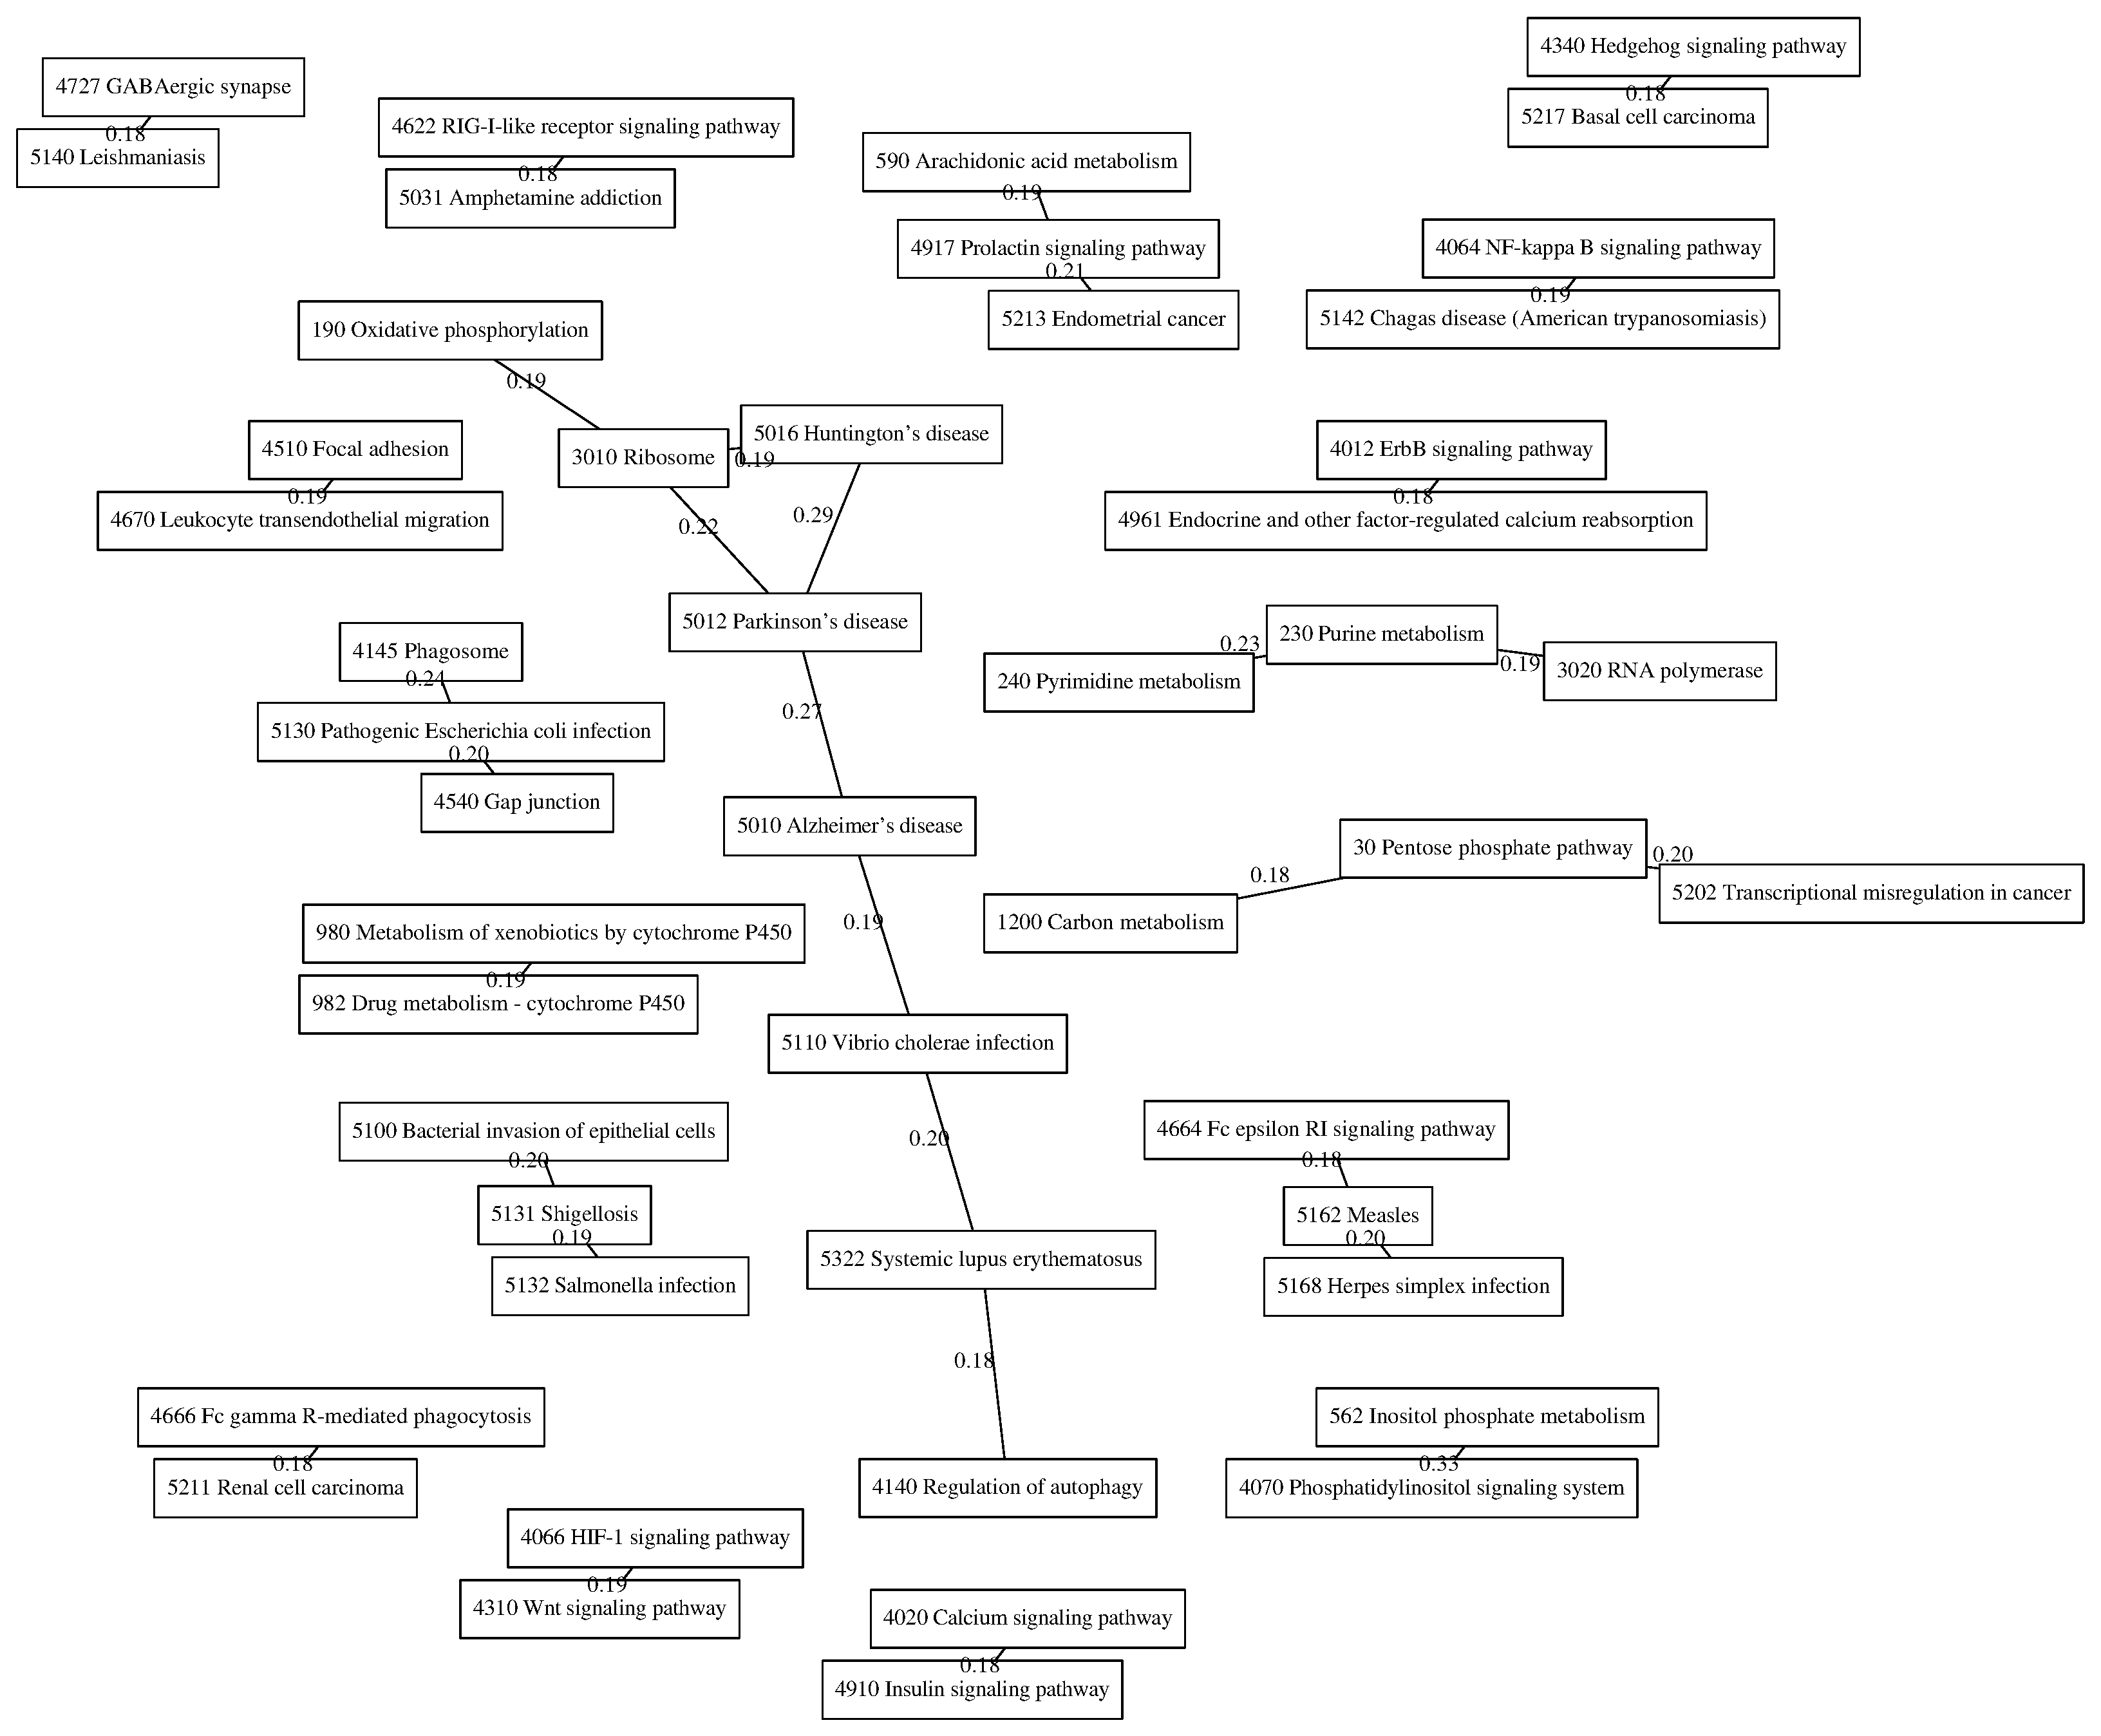
\includegraphics[width=\textwidth]{progress-report-pathways.eps}
\caption{Sample graph of pathway correlations (only pathways that have correlations greater than 0.17 are plotted). The model correctly identifies some important phenomena such as the relation between neurodegenerative diseases (Parkinson's, Huntington's, Alzheimer's), the relation between pyrine and pyrimidine (similar molecular structures) metabolism or the association of the hedgehog signalling pathway with basal cell carcinomas.}
\end{figure}

\begin{figure}[!htb]
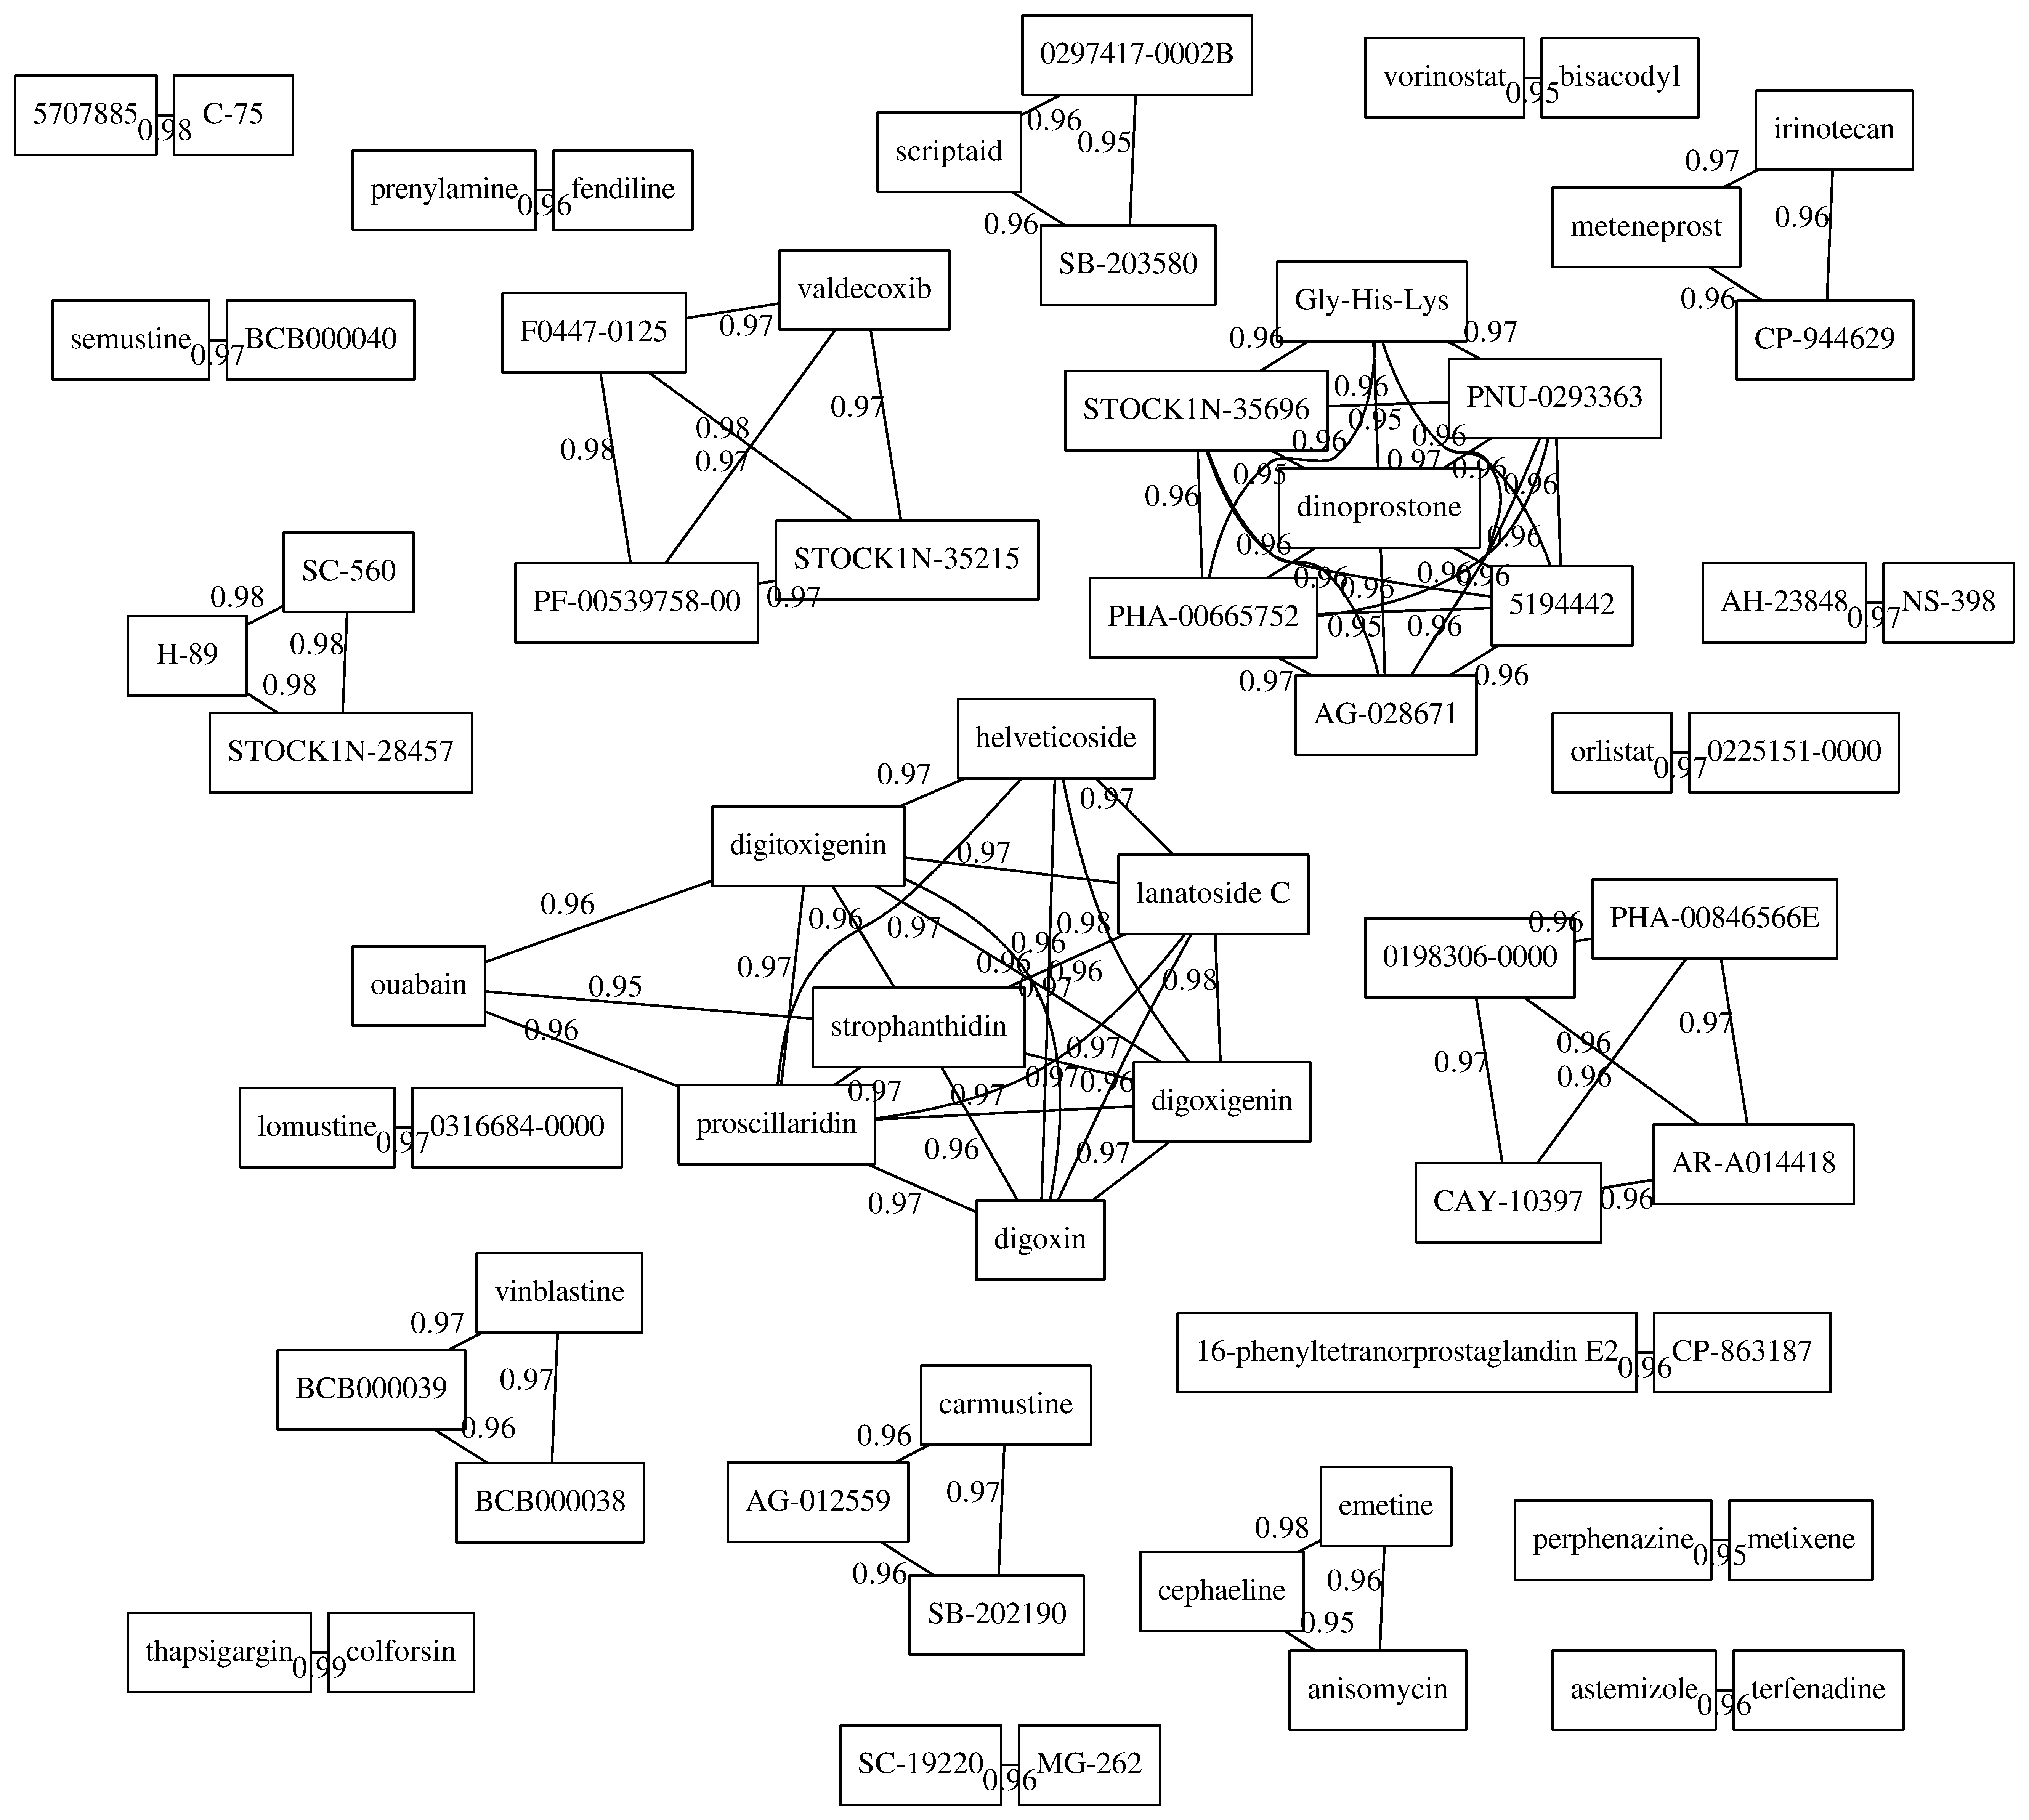
\includegraphics[width=\textwidth]{progress-report-drugs.eps}
\caption{Sample graph of the cosine similarities of drug-pathway distributions. The drugs from the sample dataset have many common pathways and so are all very similar (95\% of all drug pairs have similarity above 0.788 and 50\% above 0.880). Here, only similarities above 0.950 are plotted. Some similar drugs are identified, such as the cluster in the middle including digoxin, digoxigenin and digitoxigenin (used for cancer chemotherapy and treatment of heart conditions).}
\end{figure}

One big difficulty in evaluating the performance of the model is that of the topic identifiability. The CTM assumes that the documents are generated by first drawing a distribution of topics for every single document and then picking a topic and drawing a word from its word distribution for every word in the document. This means that the recovered topic structure is not at all guaranteed to be the same as the one used to generate the evaluation dataset. The current method used to solve this problem is using topic priors: the entries on the diagonal of the topic-word matrix are set to zero, which enforces that for every topic, there is one word that it cannot contain. However, this amount of sparsity is often not sufficient and so the evaluation process
``cheats" by considering which per-word topic distributions from the inferred and the reference topic structures are the closest and permuting the topics accordingly. Even then, there sometimes are ambiguities.

Another, more expected, difficulty was the performance of Python. Since it's an interpreted language that allows high levels of abstraction (which helped me immensely during the development of the model), it is not naturally suited for numerical computations. I used a profiler to identify performance bottlenecks in the code, which turned out to be the use of various Pythonisms like list comprehensions in the variational inference loop and rewriting them to matrix products that are evaluated by native code. Using this and some other optimisations like precomputing reused values or recycling the results of variational inference by using them to initialise the function minimiser on the next iteration, the total training time for the test dataset of similar size to the KEGG/CMap datasets that the model will be used for was brought down from 30 hours to about 8 hours.

I am now planning to:

\begin{itemize}
\item Continue evaluating the model using toy datasets: I have concerns that some of the model parameters (the mean and the covariance matrix of the global topic distributions) are not being recovered correctly.
\item Improve the performance of the training process more by, for example, trying to take advantage of the fact that the variational inference process for every document is independent and hence can be parallelized.
\item Refactor the code and implement some unit tests.
\item Start work on the dissertation and consider which extensions to the project to start implementing once the main objective has been achieved.
\end{itemize}

\end{document}